\section{Synthesis Alogrithm}
Given a set of policies, \Name creates the network forwarding model variables which abstracts the forwarding rules and reachability. For each policy, \Name adds a set of constraints on the model to the SMT Solver Z3 \cite{z3}. After all the constraints have been added, the Z3 solver returns a assignment of values for the mode satisfying the constraints. From these values, we extract the forwarding rules for each switch.
To provide support for the policies in \cref{tab:policysupport}, we use propositional logic (SAT) and linear integer arithmetic (LIA),
which are both supported by Z3. 
\subsection{Network Forwarding Model} \label{sec:fwdmodel}
We define the physical switch topology as an undirected graph $T=\{S, L\}$, where $S$ is the set of switches and $L$ is the set of links. We use the neighbour function $N(s) = \{s'\ | \ (s,s') \in L \}$ to denote the set of neighbour switches of L. The set of reachability policies is denoted as $R$ and each reachability policy $r \in R$ is
a tuple of the form $(predicate$, $src$, $dst$, $W$, $pc$) where
\begin{itemize}
\item  $predicate$ over the set of packet headers identifies the packet pertaining to $r$ ;
\item  $src,dst \in S$ are the source and destination switches;
\item $W\subseteq S$ is the (potentially empty) set of waypoints;
\item $pc \in PC$ is the packet class and is a unique integer used to identify the variables associated to $r$
\end{itemize} 
We use the notion of packet classes to distinguish reachability/waypoint policies which produces a path from other policies which impose restrictions on these paths. We define a set of packet classes $PC : [0,\lambda]$ and maps each reachability/waypoint policy to a unique integer in $PC$. In the rest of the paper, we use the term packet class to associate it to a path synthesized for a reachability/waypoint policy. 
%Assuming that the intersection of predicates is empty for policies in $R$, we create a mapping $\gamma : R \rightarrow PC$ to associate each reachability policy with a unique integer called packet class in the set $PC$. Switches $src, dst \in S$ denote the ingress and egress switches respectively for the packet class $pc = \gamma(r)$ and Genesis finds a path from $src$ to $dst$ for $pc$. If a waypoint policy is specified, $W$ is the set of switches the path from $src$ to $dst$ must traverse through in no particular order.
We define a static integer $\mu$ to be the synthetic limit for path length for any packet class, and define the set $K = [0, \mu]$ to be the set of all permissible path lengths.
\loris{why do we need this? we can enforce it with the length tactic now..} \kausik{I need for the model constraints. This is more of a synthetic limit and not to enforce any specific length properties on the path. Tactics can be used to further improve the search. if I dont have this, the model will have unbounded quantifiers. We dont want to use tactics all the time, right?}
\loris{you still can bound based on the fact that you only want acylcic paths using the number of nodes minus 1}

The key roles of the network forwarding model are abstracting the actual forwarding rules at each node and encoding the reachability of each flow. 
\begin{mydef}
\label{def:fwd}
The relation $Fwd \subseteq S \times S \times PC $ captures the forwarding rule behavior of the network. 
Concretely, $(sw_1, sw_2, pc)\in Fwd$ if 
$sw_1$ forwards packets of class $pc$ to switch $sw_2$. 
\end{mydef}
\begin{mydef}
\label{def:reach}
	The relation $Reach \subseteq N \times PC \times K$ captures the path reachability.   
	Concretely, $(sw, pc, k)\in Reach$ if 
	the switch $sw$ is reachable in the path from source switch of packet class $pc$ in exactly $k$ steps.  
\end{mydef}
For brevity, we write $Fwd(sw_1, sw_2, pc)$ for $(sw_1, sw_2, pc) $ $\in Fwd$ and similarly for the $Reach$ relation. The $Fwd$ relation can contain only connected switches in the topology. For $sw_1, sw_2$ who are not connected by a link, $\forall pc$, $(sw_1,sw_2,pc) \notin Fwd$. 

Given two concrete relations Fwd and Reach, the set $P$ of induced paths is the following, 
$sw_0 \ldots sw_k \in P$ is the path for class $pc$ iff : 
\begin{enumerate}
	\item $\forall i \in [0,k]. (sw_i, pc, i) \in Reach$
	\item $\forall i \in [0, k - 1]. (sw_i, sw_{i+1}, pc) \in Fwd$
\end{enumerate}


\begin{figure}[!th]
	\centering
	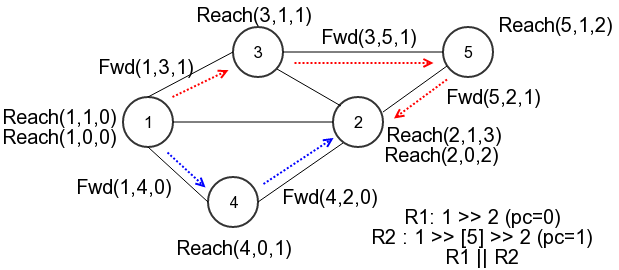
\includegraphics[width=\columnwidth]{figures/network-model-example.png}
	\caption{Values of the $Fwd$ and $Reach$ relations of the network forwarding model
		 for the policies specified in the figure. The blue and red arrows indicate the 
		 paths of packet classes 0 and 1 respectively according to the model.}
	\label{fig:model}
\end{figure}
%An example network forwarding model is shown in \cref{fig:model}. 
%%There are two reachability policies, $r1 : 1 >> [5] >> 2$ with $pc=1$ and $r2 : 1 >> 2$ with $pc=2$ and $r1$ is isolated to $r2$
%%\loris{The policies should be in the caption of the figure as well or in the figure itself}. 
%Using the value of $Fwd$ relation, we can find out paths for each packet class the forwarding rules for each switch. 

\loris{say somewhere that all those relations are encoded as propositions in SAT}
One of the decisions oriented towards performance is modelling the forwarding and relations using propositions, so that we can reduce enforcement of policies like reachability, waypoints and isolation to a Boolean Satisfiability Problem (SAT) problem\footnote{An earlier iteration of our model used \emph{uninterpreted functions} supported by Z3 and modeled reachability using recursive constraints, 
	which was slower with a greater number of constraints.}. 
The two relations for forwarding and reachability ensures we can write the constraints in a concise and intuitive manner.
\kausik{Removed the troublesome lines. Is there anything nnoteworthy with the modelling we can specify here?}
%\loris{not sure what you are trying to say with the previous 2 sentences, is it important at all?}. 
%\kausik{I am trying to motivate the requirement for the reachability relation to write constraint concisely}
%\loris{are you saying that constraints enumerating all the paths of some length would be bad? Who would do that?}

\subsection{Reachability Constraints} \label{sec:reach}
For a reachability policy $s >> d$ and packet class $pc$, the constraints added must ensure that the solution model contains a path 
from source to destination. 
One of the constraints required for this is that there must exist a forwarding rule at source to one of its neighbours, and 
these constraints
act as the base case relating the $Fwd$ and $Reach$ relations.\footnote{
	We unroll the existential quantifier $\exists n \in N(s)$ using disjuction of 
	clauses $\bigvee\limits_{n \in N(s)}$ and
	the universal quantifier $\forall n \in N(dst)$ using conjuction of clauses $\bigwedge\limits_{n \in N(dst)}$
	and stay in propositional logic.} 
\begin{equation} \label{eq:src}
	\exists n \in N(s). Fwd(s, n, pc) \wedge Reach(n, pc, 1)
\end{equation}
The base case for reachability is : $(s, pc,0) \in Reach$ . We need a path to destination, thus destination switch must be reachable for some path length : 
\begin{equation} \label{eq:dst}
	\exists k. Reach(dst, pc, k)
\end{equation}
Also, since the destination is supposed to be the last switch in the path, we add constraints
to ensure that the destination does not have forwarding rules further : 
\begin{equation}
	\forall n \in N(dst). \ \neg Fwd(dst, n, pc)
\end{equation}
For the solver to find a path, we need implication constraints propagating reachability backward from destination to source. 
If a node $n_1$ is reachable in $k$ steps, there must a node $n_2$ which is reachable in  $k-1$ steps and there exists a forwarding rule $n_2 \rightarrow n_1$.
\begin{multline} \label{eq:bckprop}
\forall n_1,k.  Reach(n_1,pc,k) \implies \exists n_2.  n_2 \in N(n_1) \wedge \\ Reach(n_2,pc,k-1) \wedge Fwd(n_2,n_1,pc)
\end{multline} 
The backward propagation is responsible for ensuring there is a topologically valid path from source to destination by using the unit clauses in \cref{eq:dst}, and finding a path from destination back to a switch $sw$ which is a neighbour of $src$. thus $Reach(sw,pc,1)$ would be true from \cref{eq:src} and the reachability policy would be satisfied. 

The above mentioned constraints are sufficient to ensure there is a path from $src$ to $dst$ for packet class $pc$ in terms of the forwarding relation $Fwd$. However, since there is no restriction on number of $Fwd$ values that can be true at a switch, we can get multiple forwarding rules at switches, and also multiple paths to the destination. Also, there can exist forwarding loops as well. From the perspective of the network model, 
this is a valid assignment as there would be atleast one path from $src$ to $dst$. 
This serves an optimization as we are able to extract a path from the solution without 
adding additional constraints to ensure the semantics of \emph{unicast} forwarding. 

For a reachability policy, we merely require to find a path from $src$ to $dst$. Thus, we extract a valid path from the model by performing a breadth-first search on the model-graph from source to destination. 
%\loris{the previous point is a bit crucial, clarify a little better} \kausik{TODO}
A directed edge exists in the model-graph : $n_1 \rightarrow n_2$ if there is forwarding rule indicated by the relation $(n_1,n_2, pc) \in Fwd$. Thus, we extract the relevant rules of the shortest path from source to destination from the model, and the additional rules obtained in the solution (extra paths, forwarding loops) are ignored.  
%\loris{we should later say that this is perhaps desirable for future extensions with broadcasting.}
\subsection{Waypoint Constraints} 
For a reachability policy with waypoints $s >> W >> d$ and packet class $pc$, we add all the constraints specified in \cref{sec:reach} to ensure the existence of a path from source to destination. To satisfy waypoint policies, we need to add constraints so that all $w \in W$ is reachable. 
\begin{equation} \label{eq:waypoints}
	\forall w \in W. \exists k. Reach(w, pc, k)
\end{equation}
However, just ensuring reachability of waypoints is not sufficient. Since, we do not have any restrictions on the count of forwarding rules for a packet class at a switch, it is possible that waypoints are reachable from the source through separate paths, and do not lie in the path from source to destination. Thus, to ensure that all waypoints are reachable in the path from source to destination, we need to add constraints on the count of forwarding rules at each switch. 

Forwarding rule constraints are to ensure that the forwarding relation $Fwd$ for a switch contains a \emph{single} switch which is a \emph{neighbour} or to no node at all (switches which are not reached in the path, and the destination will not have any forwarding rules). We define the forwarding set $FwdSet$ as follows:
\begin{equation}
	FwdSet(sw,pc) = \{n \ | \ Fwd(sw,n,pc)\}
\end{equation}
The $|A|$ function is used to the denote the size of set $A$. The constraint on the forwarding set are that the size of each set must not exceed 1 (0 or 1). The forwarding set constraint is as follows : 
\begin{equation}
		\forall sw,pc . \ |FwdSet(sw,pc)| \leq 1 \label{eq:fwdset}
\end{equation}
The forwarding set constraints ensure that the forwarding rules exist only on the path from source to destination, and no other rules exist in the solution. If a switch has a forwarding rule to  elsewhere, then it would not have a rule for the path, and the destination will not be reachable. These restrictions will also ensure there are no forwarding loops in the path. 
Since, there is only one path in the model from source and destination, and \cref{eq:waypoints} ensures that waypoints are reachable, therefore, the path from source to destination must traverse through all the waypoints. Since \cref{eq:waypoints} imposes no order on waypoint traversal, the solution will traverse the waypoints in no particular order. 

\subsection{Isolation Constraints}
For a traffic isolation policy $pc_1 || \ pc_2$ means that the paths do not share an link in the same direction in their paths, therefore, at every switch, the forwarding rules for $pc_1$ and $pc_2$ must not forward it to the same switch.  
\begin{equation}
	\forall n_1. \neg ( \exists n_2. Fwd(n_1,n_2,pc_1) \wedge Fwd(n_1,n_2,pc_2)) \label{eq:isolation}
\end{equation}
These constraints are sufficient to ensure that the packet classes $pc_1$ and $pc_2$ would be isolated. 

The isolation constraints is intuitive when coupled with the forwarding set constraints (\cref{eq:fwdset}) as the model only has forwarding rules for the path from source to destination. However, for a reachability policy without waypoints, we argue that the forwarding set constraints are not required when coupled with the isolation constraints. The reasoning behind this is that the solver would simply remove the extra forwarding rules of a packet class in the model which conflict with the other packet class, as there are no constraints which require the need of these extra forwarding rules for correctness, but are one particular solution model in the space of solutions. 

\subsection{Capacity Constraints}
%\subsubsection{Link Capacity Constraints} \label{sec:linkcap}
For a link capacity policy on the link $sw_1 \rightarrow sw_2$ with capacity $\omega$, we use the theory of integer linear arithmetic to add constraints on the link so that capacity used by the flows traversing the link does not exceed $\omega$. In terms of our model, the link capacity policy translates to constraints to ensure that the tuples $(sw_1, sw_2, pc) \in Fwd$ for $pc \in PC$ conforms to the capacity specified in the policy, as the forwarding rule $sw1 \rightarrow sw2$ means that the link is being used by the particular packet class.
 
Let $C(sw_1,sw_2,pc)$ be the cumulative capacity function of the link used by all packet classes less than equal to $pc$. Since we use integers for denoting the packet class, and thus, we have total order of the set of packet classes. We use this to create inductive constraints to sum over the set of Boolean variables $Fwd(sw_1, sw_2,pc)$. Let $PC : [0, \lambda]$ be the set of packet classes and the $W(pc)$ is the capacity of packet class $pc$ ($W$ can be uniform or non-uniform for all packet classes). 
The base case constraint for the capacity function is for $pc = 0$ (the minimum element of $PC$) :
\begin{equation}
	Fwd(sw_1, sw_2, 0) \implies C(sw_1, sw_2, 0) = W(0)
\end{equation}
\begin{equation}
	\neg Fwd(sw_1, sw_2, 0) \implies C(sw_1, sw_2, 0) = 0
\end{equation} 
The inductive constraints for the capacity function are as follows if link is used : 
\begin{multline}
	\forall pc > 0. Fwd(sw_1,sw_2,pc) \implies \\ C(sw_1, sw_2, pc) =  C(sw_1. sw_2, pc - 1) + W(pc)
\end{multline}
If the link is not used, the constraints are as follows : 
\begin{multline}
\forall pc > 0. \neg Fwd(sw_1,sw_2,pc) \implies \\ C(sw_1, sw_2, pc) =  C(sw_1. sw_2, pc - 1)
\end{multline}
If $pc$ uses the link $sw_1 \rightarrow sw_2$, we add $W(pc)$ to $C(sw_1,$ $sw_2,pc-1)$, or add 0 to it if link is not being used. Thus, we define the cumulative capacity constraints using inductive constraints. To satisfy the capacity policy, the total capacity used should not exceed input $\omega$. $\lambda$ is the greatest element in the set $PC$. 
\begin{equation}
	C(sw_1, sw_2, \lambda) \leq \omega	
\end{equation} 
We add similar constraints as described above for switch table size policies, but instead of tracking $Fwd(sw_1, sw_2,pc)$ for the link, we would have to track reachability of the path to switch $sw$, which is represented by the clause $\exists k$. $Reach($ $sw,pc,k)$.